%%%%%%%%%%%%%%%%%%%%%%% file template.tex %%%%%%%%%%%%%%%%%%%%%%%%%
%
% This is a general template file for the LaTeX package SVJour3
% for Springer journals.          Springer Heidelberg 2010/09/16
%
% Copy it to a new file with a new name and use it as the basis
% for your article. Delete % signs as needed.
%
% This template includes a few options for different layouts and
% content for various journals. Please consult a previous issue of
% your journal as needed.
%
%%%%%%%%%%%%%%%%%%%%%%%%%%%%%%%%%%%%%%%%%%%%%%%%%%%%%%%%%%%%%%%%%%%
%
% First comes an example EPS file -- just ignore it and
% proceed on the \documentclass line
% your LaTeX will extract the file if required
\begin{filecontents*}{example.eps}





%!PS-Adobe-3.0 EPSF-3.0
%%BoundingBox: 19 19 221 221
%%CreationDate: Mon Sep 29 1997
%%Creator: programmed by hand (JK)
%%EndComments
gsave
newpath
  20 20 moveto
  20 220 lineto
  220 220 lineto
  220 20 lineto
closepath
2 setlinewidth
gsave
  .4 setgray fill
grestore
stroke
grestore
\end{filecontents*}
%
\RequirePackage{fix-cm}
%
%\documentclass{svjour3}                     % onecolumn (standard format)
%\documentclass[smallcondensed]{svjour3}     % onecolumn (ditto)
%\documentclass[smallextended]{svjour3}       % onecolumn (second format)
\documentclass[twocolumn]{svjour3}          % twocolumn
%
\smartqed  % flush right qed marks, e.g. at end of proof
%
\usepackage{graphicx}
\usepackage{color}
\usepackage{listings}
\usepackage{fancyvrb}
\usepackage{url}
\usepackage{fix2col}
\usepackage{natbib}
\usepackage{epsfig}
\usepackage{algorithm}
\usepackage{algorithmic}
%\input{highlight.sty}

\lstset{
basicstyle=\ttfamily \scriptsize,
language=java,
frame=single,
stringstyle=\ttfamily,
showstringspaces=false
}

\hyphenation{sche-me}
%
% \usepackage{mathptmx}      % use Times fonts if available on your TeX system
%
% insert here the call for the packages your document requires
%\usepackage{latexsym}
% etc.
%
% please place your own definitions here and don't use \def but
% \newcommand{}{}
%
% Insert the name of "your journal" with
% \journalname{myjournal}
%
\providecommand{\e}[1]{\ensuremath{\times 10^{#1}}}
\begin{document}

\title{Effect of population size in heterogeneous and homogeneous machines in a distributed EA%\thanks{Grants or other notes
%about the article that should go on the front page should be
%placed here. General acknowledgments should be placed at the end of the article.}
}
%\subtitle{Do you have a subtitle?\\ If so, write it here}

%\titlerunning{Short form of title}        % if too long for running head

\author{P. Garc\'ia-S\'anchez \and
        J. Gonz\'alez \and
        C. Fernandes \and
        M. G. Arenas \and
		A. M. Mora \and
    P. A. Castillo \and
		J. J. Merelo
}

%\authorrunning{Short form of author list} % if too long for running head

\institute{P. Garc\'ia-S\'anchez \at
              Dept. of Computer Architecture and Computer Technology, \\
              E.T.S. Ing. Inform\'atica y Telecomunicaci\'on and CITIC-UGR\\
              University of Granada, Granada, Spain\\
              \email{pgarcia@atc.ugr.es}           %  \\
%             \emph{Present address:} of F. Author  %  if needed	
}

\date{Received: date / Accepted: date}
% The correct dates will be entered by the editor


\maketitle

\begin{abstract}
This paper shows a preliminary study about population size tuning in an distributed Genetic Algorithm. This adaptation is done taking into account the computational power of each node of an heterogeneous cluster. Same parameters are also tested in an homogeneous scientific cluster. Two problems with distinct characteristics have been tested: the linearly-solvable OneMax problem and the deceptive and multimodal MMDP functions.  Results show that setting this parameter according computational power decreases the time to obtain the optimum in both problems in heterogeneous clusters.


\keywords{
Evolutionary Algorithms \and
Service Oriented Architecture \and
Service Oriented Science \and
Web Services \and
Interoperability \and
Distributed computing}
% \PACS{PACS code1 \and PACS code2 \and more}
% \subclass{MSC code1 \and MSC code2 \and more}
\end{abstract}

\section{Introduction}
\label{sec:intro}

New trends such as Cloud Computing \cite{CLOUD}, GRID \cite{OPENSCIENCEGRID} or Service Oriented Science \cite{GLOBUS} are leading to heterogeneous computational devices working at the same time.  Moreover, many laboratories do not count with classic clusters, but the usual workstations used by scientists can behave in group as a heterogeneous cluster. Distributed Evolutionary Algorithms (dEAs) \cite{AQUIEN} have been tested successfully in these systems. 

Heterogeneous dEAs can be divided in two categories: a dEA where the parameters are different in each island (heterogeneous parameters) or the same algorithm in heterogeneous hardware. It also have been proved that this kind of algorithms are even more efficient in heterogeneous hardware configurations, than in homogeneous devices \cite{HETEROGENEOUSHARD}. This can be explained by different reasons, such as different memory access times, cache, or even implementation languages or compilers in each machine, leading to different explotation rate of the search space. The heterogeneous parameters configuration also have been proved as more efficient than a fixed set of parameters for different problems \cite{HETEROGENEOUSPARAMETERS}. Our motivation in this work is to combine both ideas adapting the population size of the islands to the heterogeneous hardware. To calculate the computational power, the algorithm is executed in each machine, and then, the total size of individuals is distributed according the number of generations attained in each node during the same time. Two different problems (MMDP and OneMax) have been used as a benchmark.


In this work, a distributed system has been developed to solve the following questions:
\begin{itemize}
 \item Can a distributed EA be adapted to take the most of the capability of a heterogeneous cluster?
 \item Does the proposed population size adaptation to the computational power scheme any effect in both systems?
 \item Is there any difference in homogeneous and heterogeneous cluster?
\end{itemize}


The rest of the work is structured as follows: after the state of
the art, we present the developed algorithms and experimental setting. 
Then, the results of the experiments are shown (Section \ref{sec:results}), followed by conclusions and suggestions for future work.


%%%%%%%%%%%%%%%%%%%%%%%%%%%%%%  SOA  %%%%%%%%%%%%%%%%%%%%%%%%%%%%%%
%
\section{State of the art}
\label{sec:soa}
%

In the field of the Evolutionary Computing there are two different approaches about the algorithm parameter setting: parameter control and parameter tuning \cite{PARAMETERTUNING}. The first one refers to set a number of parameters of an EA and to change these parameter while the algorithm is running. The parameter tuning consist in establish a good set of parameters before the run (and do not change them during runtime).

 Computational performance of nodes or network speeds can also be inherents parameter of an algorithm. In \cite{HETEROGENEOUSHARD} authors compared a distributed GA in homogeneous and heterogeneous clusters. Super-linear performance was obtained in the heterogeneous clusters, being more efficient that the same algorithm in homogeneous ones. Some authors have expanded this idea adapting the algorithm to be executed: in \cite{HYDROCM} authors presented a distributed hybrid meta-heuristic that combines GAs and Simulated Annealing (SA). Their system executes the costly algorithms (GAs) in faster nodes, and simpler meta-heuristics (SA) in slower nodes, obtaining better results than other configurations. In \cite{HETEROGENEOUSTOPOLOGY} different configurations of heterogeneous machines for a tree topology were studied. However, the heterogeneity was simulated in an homogeneous clusters with programs to add computational load. Load-balancing was also applied taking into account the computational load of the nodes in \cite{PARALLELIMPLEMENTATION}: a small benchmark was executed in all nodes at the beginning of the algorithm to distribute individuals of an Evolutionary Strategy (ES). However, there was not communication between the nodes. In the area of heterogeneous parameters, but homogeneous hardware, setting each island a random set of parameters can also increase the performance of a distributed Genetic Algorithm (dGA), as explained in \cite{HETEROGENEOUSPARAMETERS}. That model outperformed a tuned canonical dGA with the same parameters in all islands. Finally, adapting the migration period has produced better results than homogeneous periods in homogeneous clusters, as explained by \cite{HETEROGENEOUSMIGRATION}.

 Our work presents a combination of previous ideas, where a parameter tuning given by the computational cost of the machines is performed. For our knowledge, there are not works that modify parameters of the GA depending of the node where the island is being executed.


\section{Service Oriented Evolutionary Algorithms}

The EAs are a general technique for solving optimization and search problems based in the evolution of species and natural selection. These algorithms are formed by a population of possible solutions (called {\em individuals}) that competes using their {\em fitness} (quality of adaptation) with the rest of solutions. In each iteration of the algorithm (or {\em generation}) the individuals are evolved by means of selection and recombination/mutation to create a new set of candidates, until a {\em stop criterion} (i.e. number of generations) is met. Fitness function is a quality function that gives the grade of adaptation of an individual respect the others. This function is usually the problem to solve.

There are different ways to parallelize the EAs:

\begin{itemize}
\item {\em Farming model (centralized)}: A central node coordinate several slave nodes. The central node executes the EA in a sequential way, but distributes the individuals of the population to the slaves just for being evaluated.
\item {\em Island model (distributed)}: A number of nodes executes simultaneously the EA, working with different sub-populations at the same time. Each certain number of generations is interchanged (migrated) between populations.
\item {\em Cellular EAs (fine grain)}: Each node has one individual of the population, and selection and reproduction is limited with the individuals of the neighbourhood of the node. Usually a bi-dimensional grid is used for topology.
\end{itemize}

\begin{figure}
\centering
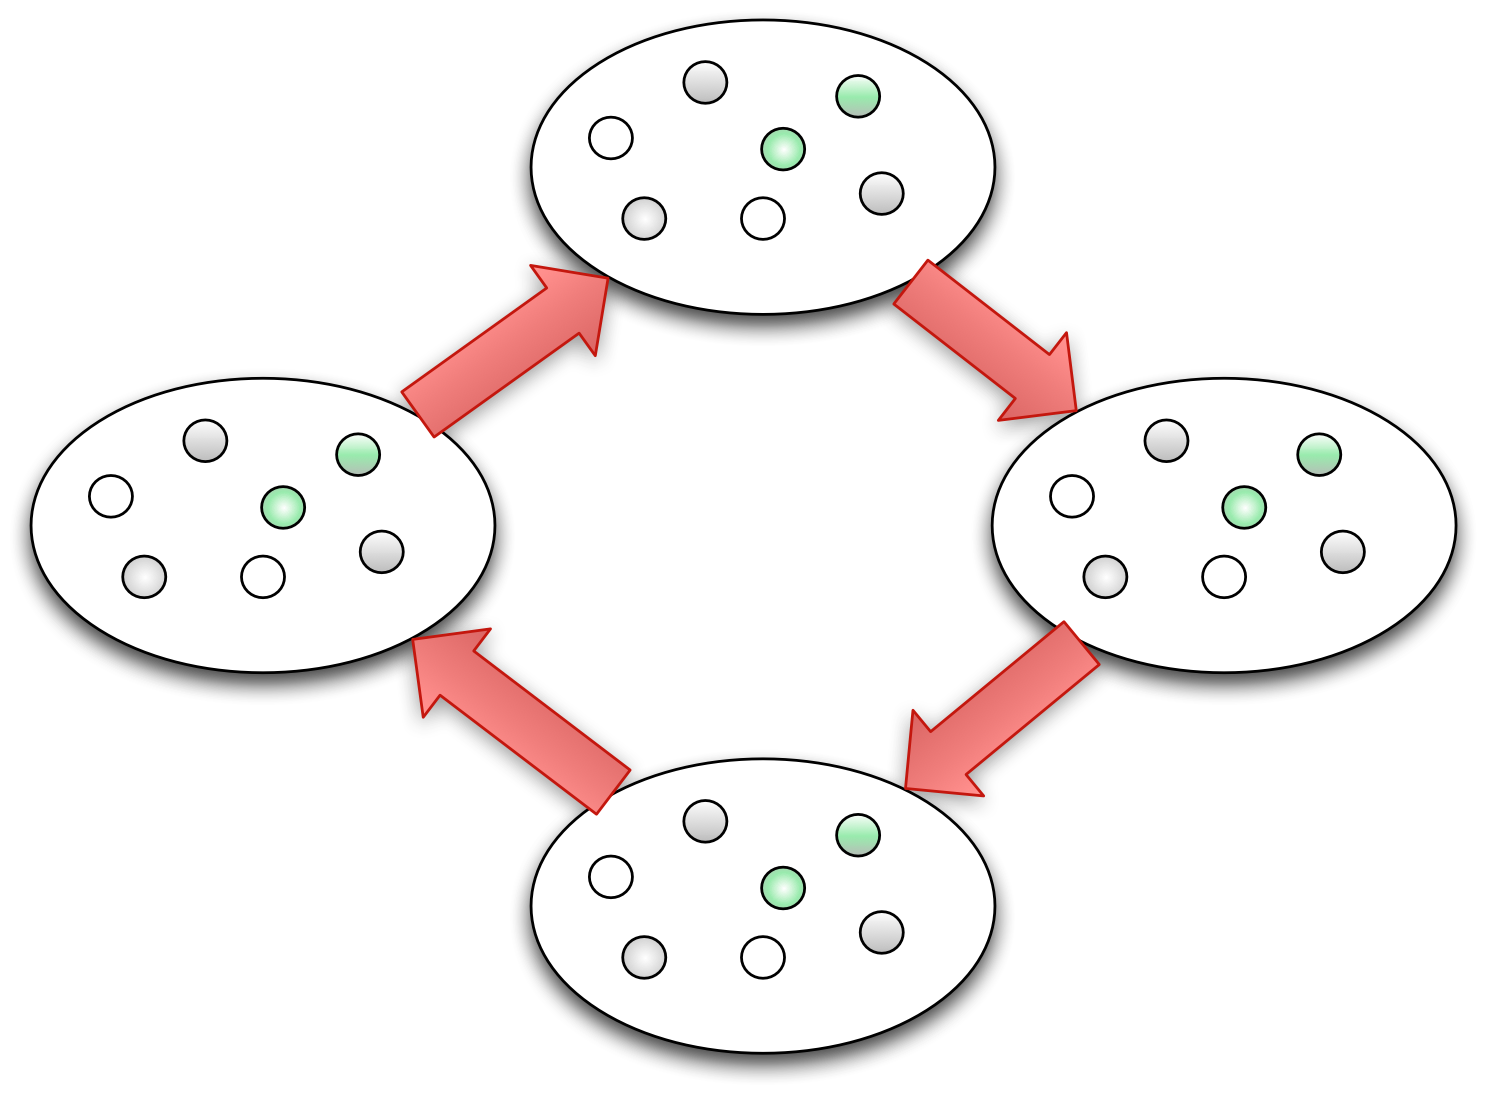
\epsfig{file=images/islands.eps, width = 7cm}
\caption{Island model using a ring topology.}
\label{fig:timeMMDP}
\end{figure}


The distributed EAs are very popular because the implementation is not complicated and they explotate a coarse grain parallelism with sporadical communications, being appropiated to be executed in distributed architectures such as clusters or GRIDs \cite{}.


As discussed in \cite{SOASOCO} the evolutionary algorithms research area is a propitious environment to migrate to SOA for several reasons: SOA fits with the genericity advantages in the development of software for EAs \citep{GENERICITY05} and adds new features, like language independence and  distribution mechanisms. Moreover, there are a large number of frameworks for EAs mostly imcompatible due to different programming languages, operating systems or communication protocols (see \cite{SURVEYMOFS} for a survey). Also, new research trends, like self-adaptation \citep{SELFSTAR}, require many changes and modifications in the algorithms behavior in real-time. And finally, the increase of technologies such as GRID and Cloud Computing \citep{CLOUD}, where the computation elements are distributed in different machines, with many operating systems and programming languages.




%%%%%%%%%%%%%%%%%%  Experiments  %%%%%%%%%%%%%%%%%%%
\section{Experimental setup}
\label{subsec:experiments}
This section presents the parameters and systems to conduce the experiments.

The algorithm to improve is a dGA. Parameters are described in Table \ref{table:parameters}. The algorithm is steady-state: the offspring is mixed with the parents and the worst individuals are removed. A ring topology is used, and the best individual is sent after a fixed number of generations of each node (64).  Two different parameter configurations have been used: 64 individuals per node (homogeneous size) and a different number of individuals proportional to the number of generations attained in this first homogeneous size execution (heterogeneous size).

Figure \ref{fig:EA} shows the pseudo-code of the used algorithm.

\begin{figure}

\begin{algorithmic}
\STATE population $\gets$ initializePopulation()
\WHILE {stop criterion not met}
    \STATE parents $\gets$ selection(population)
    \STATE offspring $\gets$ recombination(parents)
    \STATE offspring $\gets$ mutation(offspring)
    \STATE population $\gets$ population + offspring
    \IF {time to migrate}
      \STATE migrants $\gets$ selectMigrants(population)
      \STATE remoteBuffer.send(migrants)
    \ENDIF
    \IF {localBuffer.size DISTINTO zero}
      \STATE population $\gets$ population + localBuffer.read()
    \ENDIF
    \STATE population $\gets$ removeWorst(population)
\ENDWHILE

\end{algorithmic}
\caption{Pseudo-code of the used dEA.}
\label{fig:EA}
\end{figure}


\begin{table}
\centering
\caption{Parameters used.}
\begin{tabular}{|c|c|} \hline
Name & Value\\ \hline
Total individuals & 256\\ \hline
Population size in HoSi & 64 \\ \hline
Population size in HeSi & 98, 84, 66, and 8\\ \hline
Crossover type & Uniform crossover \\ \hline
Crossover rate & 0.5\\ \hline
Mutation rate & 1/genome size\\ \hline
Selection & 2-tournament \\ \hline
Replacement & Steady-state\\ \hline
Generations to migrate & 64 \\ \hline
Genome size for MMDP & 150 \\ \hline
Genome size for OneMax & 5000 \\ 

\hline\end{tabular}
\label{table:parameters}
\end{table}

The problems to evaluate are the Massively Multimodal Deceptive Problem (MMDP) \cite{goldberg92massive} and the OneMax problem \cite{ONEMAX}. Each one requires different actions/abilities by the GA at the level of population sizing, individual selection and building-blocks mixing. The MMDP
 is designed to be difficult for an EA, due to
its multimodality and deceptiveness. Deceptive problems are functions where low-order building-blocks do not combine to form higher order building-blocks. Instead, low-order building-blocks may mislead the search towards local optima, thus challenging search mechanisms. MMDP it is composed of $k$ subproblems of 6 bits each one ($s_i$). Depending of
the number of ones (unitation) $s_i$ takes the values shown in Table \ref{table:mmdp}.  

\begin{table}[h]

\centering
{%\scriptsize
\caption{ Basic deceptive bipolar function ($s_i$) for MMDP.}
\begin{tabular}{|c|c|}
\hline
\texttt{Unitation}&\texttt{Subfunction value}\\
\hline
0 & 1.000000 \\
\hline
1 & 0.000000 \\
\hline
2 & 0.360384 \\
\hline
3 & 0.640576\\
\hline
4 & 0.360384\\
\hline
5 & 0.000000\\
\hline
6 & 1.000000\\
\hline

\end{tabular}
}

\label{table:mmdp}
\end{table}
%%%%%%%%%%%%%%%%%%



The fitness value is defined as the sum of the $s_i$ subproblems with an optimum of $k$ (equation \ref{eq:mmdp}).
The search space is composed of $2^{6k}$ combinations from which there
are only $2^k$ global solutions with $22^k$ deceptive
attractors. Hence, a search method will have to find a global solution
out of $2^{5k}$ additionally to deceptiveness. In this work $k=25$. 

\begin{equation}\label{eq:mmdp}
\scriptsize
f_{MMDP}(\vec s)= \sum_{i=1}^{k} fitness_{s_i}
\end{equation}

OneMax is a simple linear problem that consists in maximising the number of ones in a binary string. That is, maximize the expression:
\begin{equation}
f_{OneMax}(\vec{x}) = \sum_{i=1}^{N}{x_{i}}
\end{equation}


To test the algorithm two different computational systems have been used: an {\em heterogeneous cluster} and an {\em homogeneous cluster}. The first one is formed by 4 different computers of our lab with different processors, operating systems and memory size. The latter is a dedicated scientific cluster formed by homogeneous nodes. Table \ref{tab:computers} shows the features of each system.

\begin{table*}
\centering{\scriptsize
\caption{Details of the clusters used.}
\begin{tabular}{|c|c|c|c|c|} \hline
Name     & Processor  & Memory  & Operating System  & Network  \\ \hline
\multicolumn{5}{|c|}{Homogeneous cluster} \\ \hline
Cluster node &  Intel(R) Xeon(R) CPU   E5320  @ 1.86GHz       & 4GB & CentOS 6.7    &   Gigabit Ethernet    \\ \hline
\hline
\multicolumn{5}{|c|}{Heterogeneous cluster} \\ \hline
N1  &  Intel(R) Core(TM)2 Quad CPU    Q6600  @ 2.40GHz    & 4GB   & Ubuntu 11.10 (64 bits)  & Gigabit Ethernet      \\ \hline
N2  &  Intel(R) Core(TM)2 Quad CPU    Q6600  @ 2.40GHz    & 4GB   & Ubuntu 11.04 (64 bits)  & Gigabit Ethernet      \\ \hline
N3  &  AMD Phenom(tm) 9950 Quad-Core Processor @ 1.30Ghz    & 3GB   & Ubuntu 10.10 (32 bits)  & 100MB Ethernet      \\ \hline
N4  &  Intel (R) Pentium 3 @ 800MHz               & 768 MB  & Ubuntu 10.10 (32 bits)  &   10MB Ethernet     \\ \hline
\end{tabular}
}
\label{tab:computers}
\end{table*}

Because the operating system and architecture heterogeneity the ANONYMOUS framework \cite{OSGILIATH}, based in Java, has been used. This is a service-oriented evolutionary framework that automatically configures services to use and be used in a local network. In this case, each node offers a migration buffer to accept foreign individuals. Also, to avoid bottlenecks in distributed executions, asynchronous communication has been provided to avoid idle time using reception buffers (that is, the algorithm does not wait until new individuals arrive). This kind of communication offers excellent performance when working with different nodes and operating systems, as demonstrated by \cite{HETEROGENEOUSHARD}. The transmission mechanism is based in ECF Generic server (over TCP)\footnote{\url{http://www.eclipse.org/ecf/}}. The source code of the algorithms used in this work is available in \url{http://anonymous} under a GPL V3 License.

Each different configuration has been tested 30 times. Acronyms for each configuration are HoSi (homogeneous population size), HeSi (heterogeneous population size), HoHa (homogeneous hardware) and HeHa (heterogeneous hardware). 

The number of individuals in each node of the HeSi configuration is proportional to the average number of generations obtained in the nodes of the HoSi/HeHa configuration for the MMDP problem. Thus, the HeSi configuration uses 98, 84, 66, and 8 individuals (from N1 to N4). Note that, having two nodes with the same processors and memory (N1 and N2), they have different computational power.
%%%%%%%%%%%%%%%%%%  Results  %%%%%%%%%%%%%%%%%%%

\section{Results}
\label{sec:results}

The objetives of the parallel programming are to tackle large computational problems, increase the performance of algorithms in a finite time, or reduce time. In this work we focus in the last objective.
As claimed by \cite{EVALUATIONPARALLEL} the number of evaluations can be misleading in the parallel algorithms area. In our case, for example, the evaluation time is different in each node of the heterogeneous cluster, and the real algorithm speed could not be reflected correctly. However, the number of evaluations has been added in this section to better understand the results. Also, the total number of generations, and the maximum number of generations of the slower of the four nodes are shown. It is difficult to compare between the HoHa and HeHa for the same reasons: the evaluation time is different in each system (and also in each node).

\subsection{MMDP Problem}

Table \ref{tab:resultsMMDP} shows the results for the MMDP problem. These results are also shown in the boxplots of the Figure \ref{fig:evalsMMDP} (evaluations) and Figure \ref{fig:timeMMDP} (time). Table \ref{tab:significance} shows the statistical significance of the results. First, a Kolmogorov-Smirnov test is performed to asset the normality of the distributions. If the results fit a normal distribution, then a Student's T-Test is calculated. Otherwise, the non-parametric test Wilcoxon signed rank is applied (see \cite{TUTORIAL} for a tutorial for comparing EAs).

 In the HeHa system, adapting the population to the computational power of each node makes the algorithm to end significantly faster, but with the same number of evaluations (with no statistical significance). This can be explained because the evaluation time is different in all nodes. On the other hand, in the HoHa system, setting the same population sizes makes no difference in time and evaluations, that is, changing this parameter does not influence the performance of the algorithm. 

\begin{table*}
\centering
\caption{Results for the MMDP problem.}
\begin{tabular}{|c|c|c|c|c|} \hline
Configuration & Max. generations      & Total generations     &   Total evaluations     & Time (ms) \\ \hline
HoSi/HeHa   & 146401,48 $\pm$ 65699,69  & 380967,25 $\pm$ 168568,84 & 24382416,51 $\pm$ 10788405,87 & 136914,03 $\pm$ 60028,48\\ \hline
HeSi/HeHa   & 96051,5 $\pm$ 45110,90  & 289282,3  $\pm$ 135038,10 & 21784528,66 $\pm$ 10161989,38 & 109875,76 $\pm$ 49185,51\\ \hline \hline
HoSi/HoHa   & 107334,46 $\pm$ 78167,19  & 393119,86 $\pm$ 241835,27 & 25273201,06 $\pm$ 15386663,12 & 237759,43 $\pm$ 178709,86\\ \hline
HeSi/HoHa   & 149732,6 $\pm$ 81983,74 & 438171,16 $\pm$ 240169,19 & 24430043,46 $\pm$ 13395037,34 & 245776,93 $\pm$ 134715,52\\ \hline

\end{tabular}
\label{tab:resultsMMDP}
\end{table*}
%%%%CAMBIAR EL ORDEN!!!

%MMDP EVALS
%HomoSizeHomoHard-HomoSizeHeteroHard 22.83333     23.69541      FALSE
%HomoSizeHomoHard-HeteroSizeHomoHard  4.90000     23.69541      FALSE
%HomoSizeHomoHard-HeteroSizeHeteroHard 37.53333     23.69541       TRUE
%HomoSizeHeteroHard-HeteroSizeHomoHard 27.73333     23.69541       TRUE
%HomoSizeHeteroHard-HeteroSizeHeteroHard 14.70000     23.69541      FALSE
%HeteroSizeHomoHard-HeteroSizeHeteroHard 42.43333     23.69541       TRUE





\begin{figure}
\centering
\epsfig{file=images/timeMMDP.eps, width = 9cm}
\caption{Time to obtain the optimum in the MMDP problem (milliseconds). White is the heterogeneous cluster and gray the homogeneous one.}
\label{fig:timeMMDP}
\end{figure}

\begin{figure}
\centering
\epsfig{file=images/evalsMMDP.eps, width = 9cm}
\caption{Number of evaluations for MMDP problem. White is the heterogeneous cluster and gray the homogeneous one.}
\label{fig:evalsMMDP}
\end{figure}

To see the difference of how the evolution is being performed, the average fitness in each node of HeHa is shown in Figures \ref{fig:hosiheha} and \ref{fig:hesiheha}. As can be seen, with the HeSi (Figure \ref{fig:hesiheha}), the local optima are overtaken in less time than HoSi (Figure \ref{fig:hosiheha}).  This can be explained because in HeSi, the migration from N4 to N1 is performed faster, adding more heterogeneity to the whole system. White gaps in the figures are the time where the nodes are sending the individual to other nodes (not while they are receiving them). In the HoHa systems, the populations are evolved at the same time, being the average fitness similar in all nodes during all run. % The natural migration period variation from a processor to another is also giving more diversity to the populations that migrating at the same time of the homogeneous


\begin{figure*}
\centering
\epsfig{file=images/homosize_heterohard_avg.eps, angle=-90, width = 13cm}
\caption{Average fitness in the first 1000 milliseconds of execution of the four nodes of the heterogeneous cluster with the same population sizes (HoSi/HeHa) for the MMDP problem.}
\label{fig:hosiheha}
\end{figure*}

\begin{figure*}
\centering
\epsfig{file=images/heterosize_heterohard_avg.eps, angle=-90, width = 13cm} %Era 9
\caption{Average fitness in the first 1000 milliseconds of execution of the four nodes of the heterogeneous cluster with different population sizes (HeSi/HeHa) for the MMDP problem.}
\label{fig:hesiheha}
\end{figure*}



\subsection{OneMax Problem}

Results for this problem are shown in Table \ref{tab:onemaxresults} and Figures \ref{fig:evalsOneMax} and \ref{fig:timeOneMax}. In this problem, adapting the population sizes decreases significantly the time for solving in the heterogeneous cluster, and, as before, the number of evaluations remains the same (see statistical significance in Table \ref{tab:significance}). In the homogeneous system, the effect of changing the population sizes is more evident, and this time the evaluations (and therefore, the time) are reduced (both significally). 

The efficiency on OneMax problems depends more on the ability to mix the building-blocks, and less on the genetic diversity and size of the population (as with MMDP). No genetic diversity is particularly required. When properly tuned, a simple Genetic Algorithm is able to solve OneMax in linear time. Sometimes, problems like OneMax are used as control functions, in order to check if very efficient algorithms on hard functions fail on easier functions. As can be seen in Figure \ref{fig:gensonemaxhomosize}, the HoSi/HeHa, the average fitness of all populations are increasing in linear way. However, the lower processor evaluates extremely less times.  On the other side, in Figure \ref{fig:gensonemaxheterosize}, the adaptation of the population size makes that lower processors increase the number of evaluations, but the average fitness is also maintained in linear way (and in smaller increase rate) between migrations. However, the other processors are still spending more number of evaluations. That is the reason why the number of evaluations is higher in HeHa, and lower in HoHa. Computational time is more efficiently used in faster nodes, having more chance to mix the individuals. Also, because the larger size of the individuals in the OneMax problem (5000 bits vs. 150), the transmission time is larger, (white gaps in the figures). That also implies for N4 send their best individual to N1 in a extremely large time when using HoSi (each 64 generations).

\begin{table*}
\centering
\caption{Results for the OneMax problem.}
\begin{tabular}{|c|c|c|c|c|} \hline
Configuration & Max. generations      & Total generations     &   Total evaluations     & Time (ms) \\ \hline
HoSi/HeHa   & 4739,41$\pm$  305,32    & 12081,51$\pm$ 776,35  & 773729,03$\pm$  49686,72  & 72152,32$\pm$ 4994,71 \\ \hline
HeSi/HeHa   & 3438,03 $\pm$ 149,47 &  11277,33$\pm$ 471,77 &  794157,73$\pm$  31843,10  & 61870,2 $\pm$ 2518,74 \\ \hline \hline
HoSi/HoHa   & 3133,36$\pm$  101,70  & 12347,83$\pm$ 394,99  & 790773,33$\pm$  25279,52  & 62105,03$\pm$ 1964,75 \\ \hline
HeSi/HoHa   & 13897,86$\pm$ 625,27    & 20725,63$\pm$ 929,43  & 651952,8 $\pm$  29114,54  & 56120,53$\pm$ 2491,92 \\ \hline
\end{tabular}
\label{tab:onemaxresults}
\end{table*}

\begin{figure}
\centering
\epsfig{file=images/evalsOneMax.eps, width = 9cm}
\caption{Number of evaluations for OneMax problem. White is the heterogeneous cluster and gray the homogeneous one.}
\label{fig:evalsOneMax}
\end{figure}

\begin{figure}
\centering
\epsfig{file=images/timeOneMax.eps, width = 9cm}
\caption{Time to obtain the optimum in the OneMax problem (milliseconds). White is the heterogeneous cluster and gray the homogeneous one.}
\label{fig:timeOneMax}
\end{figure}

\begin{figure*}
\centering
\epsfig{file=images/homosize_heterohard_onemax_avg.eps, angle=-90, width = 13cm}
\caption{Average fitness in the first 3000 milliseconds of execution of the four nodes of the heterogeneous cluster with the same population sizes (HoSi/HeHa) for the OneMax problem.}
\label{fig:gensonemaxhomosize}
\end{figure*}

\begin{figure*}
\centering
\epsfig{file=images/heterosize_heterohard_onemax_avg.eps, angle=-90, width = 13cm}
\caption{Average fitness in the first 3000 milliseconds of execution of the four nodes of the heterogeneous cluster with different population sizes (HeSi/HeHa) for the OneMax problem.}
\label{fig:gensonemaxheterosize}
\end{figure*}

\begin{table*}
\centering
\caption{Statistical significance of the results.}
\begin{tabular}{|c|c|c|c|c|} \hline
Configuration     &Normal &Test applied     &P-value & Significant difference?\\ \hline
\multicolumn{5}{|c|}{Time for MMDP} \\ \hline
HoSi/HeHa vs HeSi/HeHa  &Yes  &T-Test     & 0.032    & Yes \\ \hline
HoSi/HoHa vs HeSi/HoHa  &No   &Wilcoxon   &0.567   & No \\ \hline \hline
\multicolumn{5}{|c|}{Evaluations for MMDP}  \\ \hline
HoSi/HeHa vs HeSi/HeHa  &Yes  &T-Test     &0.231  & No \\ \hline
HoSi/HoHa vs HeSi/HoHa  &No   &Wilcoxon   &0.958  & No \\ \hline \hline
\multicolumn{5}{|c|}{Time for OneMax} \\ \hline
HoSi/HeHa vs HeSi/HeHa  & Yes & T-Test    &  9\e{-15} & Yes \\ \hline
HoSi/HoHa vs HeSi/HoHa  & No  & Wilcoxon    &   1\e{-6} & Yes \\ \hline \hline
\multicolumn{5}{|c|}{Evaluations for OneMax}  \\ \hline
HoSi/HeHa vs HeSi/HeHa  & No  & Wilcoxon    & 0.14    & No\\ \hline
HoSi/HoHa vs HeSi/HoHa  & Yes & T-Test    & 2\e{-27}  & Yes \\ \hline

\end{tabular}
\label{tab:significance}
\end{table*}

\subsection{Analysis of the time}

This sub-section analyses the time of each section of the EA in ... blablabla.

\begin{table*}
\centering
\caption{Times of the sections of the algorithm for the MMDP problem.}
\begin{tabular}{|c|c|c|c|c|c|} \hline
\multicolumn{6}{|c|}{Homogeneous Size} \\ \hline
Node	& Selection		& Recombination		& Mutation		& Replacement		& Migration	        \\ \hline
HeN1	& 0,011 $\pm$ 0,023	& 0,181	$\pm$ 0,149	& 0,269	$\pm$ 0,064	& 0,429	$\pm$ 4,873	& 23,097 $\pm$ 	31,917 \\ \hline
HeN2	& 0,015	$\pm$ 0,009	& 0,231	$\pm$ 0,116	& 0,357	$\pm$ 0,043	& 0,449	$\pm$ 5,214	& 22,928 $\pm$ 	35,187 \\ \hline
HeN3	& 0,017	$\pm$ 0,016	& 0,291	$\pm$ 0,132	& 0,372	$\pm$ 0,117	& 0,655	$\pm$ 6,533	& 36,139 $\pm$ 	38,434 \\ \hline
HeN4	& 0,257	$\pm$ 0,371	& 5,381	$\pm$ 14,941	& 2,556	$\pm$ 1,611	& 2,400	$\pm$ 5,588	& 43,490 $\pm$ 	9,475 \\ \hline \hline
HoN1	& 0,017	$\pm$ 0,016	& 0,268	$\pm$ 0,555	& 0,405	$\pm$ 0,051	& 0,913	$\pm$ 1,350	& 8,428	$\pm$ 5,276 \\ \hline
HoN2	& 0,017	$\pm$ 0,029	& 0,267	$\pm$ 0,409	& 0,405	$\pm$ 0,037	& 0,911	$\pm$ 1,419	& 8,441	$\pm$ 4,869 \\ \hline
HoN3	& 0,017	$\pm$ 0,021	& 0,272	$\pm$ 0,589	& 0,404	$\pm$ 0,249	& 0,914	$\pm$ 1,420	& 8,177	$\pm$ 4,072 \\ \hline
HoN4	& 0,017	$\pm$ 0,010	& 0,247	$\pm$ 0,479	& 0,356	$\pm$ 0,042	& 0,857	$\pm$ 1,636	& 8,284	$\pm$ 4,770 \\ \hline
\multicolumn{6}{|c|}{Heterogeneous Size} \\ \hline									
Node	& Selection		& Recombination		& Mutation		& Replacement		& Migration	\\ \hline
HeN1	& 0,016	$\pm$ 0,012	& 0,259	$\pm$ 0,402	& 0,384	$\pm$ 0,086	& 0,435	$\pm$ 4,760	& 22,389 $\pm$ 	31,184 \\ \hline
HeN2	& 0,019	$\pm$ 0,015	& 0,297	$\pm$ 0,408	& 0,467	$\pm$ 0,256	& 0,464	$\pm$ 4,956	& 23,044 $\pm$ 	32,704 \\ \hline
HeN3	& 0,017	$\pm$ 0,016	& 0,303	$\pm$ 0,522	& 0,376	$\pm$ 0,118	& 0,634	$\pm$ 6,156	& 34,804 $\pm$ 	35,557 \\ \hline
HeN4	& 0,055	$\pm$ 0,161	& 0,769	$\pm$ 4,056	& 0,361	$\pm$ 0,653	& 1,957	$\pm$ 8,160	& 43,300 $\pm$ 	26,672 \\ \hline \hline
HoN1	& 0,025	$\pm$ 0,017	& 0,389	$\pm$ 0,676	& 0,603	$\pm$ 0,060	& 0,929	$\pm$ 1,300	& 8,396	$\pm$ 4,147 \\ \hline
HoN2	& 0,022	$\pm$ 0,017	& 0,362	$\pm$ 0,523	& 0,530	$\pm$ 0,228	& 0,921	$\pm$ 1,265	& 8,498	$\pm$ 4,694 \\ \hline
HoN3	& 0,017	$\pm$ 0,011	& 0,259	$\pm$ 0,558	& 0,403	$\pm$ 0,050	& 0,916	$\pm$ 1,409	& 8,250	$\pm$ 4,516 \\ \hline
HoN4	& 0,003	$\pm$ 0,005	& 0,039	$\pm$ 0,333	& 0,054	$\pm$ 0,029	& 0,836	$\pm$ 1,513	& 8,089	$\pm$ 4,602 \\ \hline
\end{tabular}
\label{tab:mmdptimes}
\end{table*}

\begin{table*}
\centering
\caption{Times of the sections of the algorithm for the MMDP problem.}
\begin{tabular}{|c|c|c|c|c|c|} \hline
\multicolumn{6}{|c|}{Homogeneous Size} \\ \hline
Node	& Selection		& Recombination		& Mutation		& Replacement		& Migration	        \\ \hline
HeN1	& 0,014	$\pm$ 0,016	& 4,063	$\pm$  3,290		& 7,826		$\pm$  	0,513	& 5,300 $\pm$ 62,474 &	328,262	$\pm$ 387,402 \\ \hline
HeN2	& 0,015	$\pm$ 0,019	& 4,221	$\pm$ 3,251			& 	8,325	$\pm$  	1,348	& 6,390	$\pm$ 71,926 &	398,119	$\pm$ 428,012 \\ \hline
HeN3	& 0,020	$\pm$ 0,022	& 8,896	$\pm$ 3,561			& 12,289	$\pm$  	0,393	& 6,505	$\pm$ 77,069 &	410,141	$\pm$ 480,055 \\ \hline
HeN4	& 0,362	$\pm$ 0,920	& 341,888$\pm$ 381,390		& 97,075	$\pm$  	119,923	& 3,638	$\pm$ 14,627 &	112,680	$\pm$ 43,776 \\ \hline
HoN1	& 0,021	$\pm$ 0,013	& 6,181	$\pm$ 2,386			& 11,545	$\pm$  	0,468	& 1,506	$\pm$ 3,642	& 28,355	$\pm$ 8,606 \\ \hline
HoN2	& 0,021	$\pm$ 0,013	& 6,685	$\pm$ 1,927			& 11,779	$\pm$  	1,242	& 1,364	$\pm$ 2,437	& 18,034	$\pm$ 7,422 \\ \hline
HoN3	& 0,022	$\pm$ 0,016	& 6,154	$\pm$ 2,238			& 11,585	$\pm$  	0,506	& 1,363	$\pm$ 2,437	& 18,948	$\pm$ 6,072 \\ \hline
HoN4	& 0,021	$\pm$ 0,007	& 6,124	$\pm$ 2,346			& 11,560	$\pm$  	0,519	& 1,314	$\pm$ 2,308	& 17,920	$\pm$ 4,816 \\ \hline
\multicolumn{6}{|c|}{Heterogeneous Size} \\ \hline									
Node	& Selection		& Recombination		& Mutation		& Replacement		& Migration	\\ \hline
HeN1	& 0,017	$\pm$ 0,002	& 5,955	$\pm$ 3,569	    	& 11,761	$\pm$ 0,500		& 1,000	$\pm$ 11,748 & 50,470 $\pm$ 81,518 \\ \hline
HeN2	& 0,015	$\pm$ 0,002	& 5,448	$\pm$ 3,102			& 10,879	$\pm$ 1,545		& 0,972	$\pm$ 11,253 & 48,942 $\pm$ 77,468 \\ \hline
HeN3	& 0,016	$\pm$ 0,003	& 8,733	$\pm$ 2,180			& 11,672	$\pm$ 0,870		& 1,113	$\pm$ 7,352	& 59,133 $\pm$ 	8,825 \\ \hline
HeN4	& 0,040	$\pm$ 0,035	& 17,943 $\pm$ 23,543		& 10,751	$\pm$ 1,683		& 2,144	$\pm$ 9,815	& 76,816 $\pm$ 15,500 \\ \hline
HoN1	& 0,032	$\pm$ 0,014	& 9,587 $\pm$ 	5,671		& 17,506	$\pm$ 1,083		& 1,482	$\pm$ 2,245	&17,121  $\pm$ 	6,302 \\ \hline
HoN2	& 0,027	$\pm$ 0,015	& 8,826	$\pm$ 5,850			& 15,262	$\pm$ 1,091		& 1,422	$\pm$ 2,766	&17,831	 $\pm$ 14,158 \\ \hline
HoN3	& 0,021	$\pm$ 0,013	& 6,108	$\pm$ 3,461			& 11,655	$\pm$ 0,534		& 1,365	$\pm$ 2,294  &17,440  $\pm$ 	6,578 \\ \hline
HoN4	& 0,004	$\pm$ 0,002	& 0,807	$\pm$ 0,749			& 1,653		$\pm$ 0,051		& 0,922	$\pm$ 2,672	&17,411	 $\pm$ 12,177 \\ \hline
\end{tabular}
\label{tab:mmdptimes}
\end{table*}

\section{Conclusions}
New trends, such as Cloud Computing or Service Oriented Architecture are providing a massively amount of heterogeneous computational devices. This work shows a preliminary study about adapting the population size of an EA to computational power of different nodes in an heterogeneous cluster. Results show that adapting the population size decrease the execution time significantly in heterogeneous clusters, while changing this parameter in homogeneous clusters not always performs better. This is a promising start for adapting EAs to the computational power of each execution node.

In future work a scalability study will be performed, with more computational nodes and larger problem instances. Also, other parameters such as migration rate or crossover probability will be adapted to the execution nodes. This studies will lead to automatic adaptation during runtime, with different nodes entering or exiting in the topology during the algorithm execution or adapting to the current load of the system.



\begin{acknowledgements}
This work has been supported in part by FPU research grant AP2009-2942 and projects AmIVital (CENIT2007-1010), EvOrq (TIC-3903), and TIN2011-28627-C04-02.
\end{acknowledgements}

\bibliographystyle{spbasic}
\bibliography{heterogeneous} 




\end{document}
% end of file template.tex

